\documentclass{aa}
\usepackage[varg]{txfonts}
\usepackage[separate-uncertainty=true]{siunitx}
\usepackage[version=3]{mhchem}

\sisetup{
    range-units         = brackets,
}


\def\eps{\varepsilon}
\def\aap{A\&A}
\def\apj{ApJ}
\def\apjs{ApJS}
\def\apjl{ApJL}
\def\mnras{MNRAS}
\def\aj{AJ}
\def\nat{Nature}
\def\aaps{A\&A Supp.}
\def\prd{Phys. Rev. D}
\def\prl{Phys. Rev. Lett.}
\def\araa{ARA\&A}       % Annual Review of Astron and Astrophys

\begin{document}


\title{NIR spectroscopy of the Sun and HD20010}
\subtitle{Compiling a new linelist in the NIR}


\author{D.~T.~Andreasen\inst{1,2}
    \and S.~G.~Sousa.\inst{1,2}
    \and E.~Delgado Mena.\inst{1,2}
    \and N.~C.~Santos.\inst{1,2}}


\institute{
Instituto de Astrof\'isica e Ci\^encias do Espa\c{c}o, Universidade do Porto, CAUP, Rua das
Estrelas, PT4150-762 Porto, Portugal
    \email{daniel.andreasen@astro.up.pt}
\and
Departamento de F\'isica e Astronom\'ia, Faculdade de Ci\^encias, Universidade do Porto, Portugal
}







\date{Received ...; accepted ...}

\abstract{}{}{}{}



\keywords{data reduction: high resolution spectra -- data reduction: low
    resolution spectra -- stars individual: HD20010 -- stars individual: Sun}
\maketitle



\section{Introduction}
\label{sec:introduction}

Effective surface temperature ($T_\mathrm{eff}$), surface gravity
($\log g$), and metallicity ([Fe/H], where iron is normally used
as a proxy) are fundamental atmospheric parameters necessary to
characterise a star, as well as to determine other indirect fundamental
parameters, such as mass, radius, and age from stellar evolutionary
models \citep{Girardi2000}.

Precise and accurate stellar parameters are also essential in
exoplanet searches. Planetary radius and mass are mainly found from
lightcurve analysis and radial velocity analysis, respectively. The
determination of the mass of the planet implies a knowledge of the
stellar mass, while the measurement of the radius of the planet
is dependent on our capability to derive the radius of the star
\citep{Ammler2009,Torres2008,Torres2012}.

The derivation of precise stellar atmospheric parameters is however not
a simple task. Different approaches often lead to discrepant results
\citep[see e.g.][]{Santos13}. Interferometry, usually only possible for
bright nearby stars, are usually considered as an accurate method to
derive stellar radii \citep[e.g.][]{Boyajian2012}. Another technique
is asteroseismology were stellar pulsation observed at the surface
originates from deeper layers of a star, and therefore reveals the inner
structure. From asteroseismology it is possible to (in a relatively
easy way) measure the surface gravity and mean density, and therefore
\citep{Kjeldsen1995} calculate the mass and radius. This technique has
been tested in great extent for solar like stars and red giants from
ground based observations and since the launch of the \emph{Kepler}
mission and the CoRoT mission \citep{Michel2008,Huber2011,Huber2012}.
\cite{Campante2015} is an example of usage of asteroseismology for
characterization of planetary system.

As key to all these approaches is a correct determination
of the effective temperature. In that respect, the
IRFM is usually considered as one of the most reliable
\citep{Blackwell1977,Ramirez2005b,Casagrande2010}. However, these
methods needs a priori knowledge of the bolometric flux, surface gravity
and stellar metallicity.

Finally, the use of high resolution spectroscopy, together with stellar
atmospheric models, is also often used to derive, simultaneously,
all the key atmospheric stellar parameters. The chosen procedure
often depends on the quality of the spectra, their resolution, and
wavelength region. For low resolution, below 20000, it is preferred
to fit the overall observed spectrum with a synthetic one \citep[see
e.g.][]{Onehag2012}. For higher resolution at low rotational velocities
(below 10 to 15 \si{km/s}) we can use the equivalent width (EW) method
(for details see Section~\ref{sec:method}). To use this method the key
is to resolve all lines we are interested in. For FGK stars we can use
optical spectra since these stars are the brightest in this wavelength
domain. However, when we move to the cool M stars the near infrared
(NIR) is preferred because of the higher brightness and less molecular
line blending in the spectra.

Derivation of stellar atmospheric parameters from high
resolution spectra in the optical is now a standard way
to obtain those parameters. With the advancement of NIR
instruments, we will now be able to explore a new domain. At
the moment the GIANO spectrograph installed at TNC is already
available\footnote{\url{http://www.bo.astro.it/giano/GIANO/GIANO_Overvie
w.html}}, as well as the IRD spectrograph installed at Subaru
\citep{IRD}. Furthermore, the CRIRES spectrograph at VLT is being
updated to
CRIRES+\footnote{\url{http://www.eso.org/sci/facilities/develop/instruments/crires_up.html}},
CARMENES for the 3.5 m telescope at Calar Alto Observatory \citep{CARMENES}, and
SPIROU at CFHT\footnot{\url{http://cfht.hawaii.edu/en/news/SPIRou/}}. The spectral
resolution for these spectrographs range between 50000 and 100000.

In this paper we want to explore the possibility to create a
line list of iron lines in the NIR which can be applied for FGK
stars in a consistent way. The paper is organized as follows:
In Section~\ref{sec:method} we present the method for deriving
parameters with the equivalent width method for an iron line list.
In Section~\ref{sec:results} we present the results for the derived
parameters for the Sun and HD20010.



% \begin{table*}[tb!]
%     \caption{Four high-resolution NIR spectrographs adequate for our proposed
%         methodology}
%     \label{tab:spectrograph}
%     \centering
%     \begin{tabular}{llllll}
%       \hline\hline
%         Spectrograph & Resolution   & Wavelength coverage               & First light & References \\
%       \hline
%         CRIRES+      & 50000-100000 & YJHKLM                            & 2017        & 1 \\
%         CARMENES     & 82000        & \SIrange{0.55}{1.7}{\micro\meter} & 2015        & \cite{CARMENES} \\
%         SPIRou       & 75000        & YJHK                              & 2017        & 2 \\
%         IRD          & 70000        & \SIrange{0.97}{1.75}{\micro\meter}& 2014        & \cite{IRD} \\
%         GIANO        & 50000        & \SIrange{0.90}{2.5}{\micro\meter} & 2012        & 3 \\
%       \hline
%     \end{tabular}
%     \tablebib{
%         (1)~\url{http://www.eso.org/sci/facilities/develop/instruments/crires_up.html};
%         (2)~\url{http://cfht.hawaii.edu/en/news/SPIRou/};
%         (3)~\url{http://www.bo.astro.it/giano/GIANO/GIANO_Overview.html}
%     }
% \end{table*}






\section{Method}
\label{sec:method}

The two most widely used methods for deriving stellar atmosphere
parameters from a spectrum are spectral synthesis and the equivalent
width method. The spectral synthesis method compares a synthetic
spectrum with an observed spectrum and by minimization procedure the
best fit is found between the synthetic spectrum and the real spectrum
\citep[see e.g.][]{Valenti2005,Onehag2012}. When the minimization
procedure reaches a minimum, the final atmospheric parameters are found.

The other method is the equivalent width (EW) method, which we use in this
work. With this method the EWs are measured for all lines in a line list. The
EW is given as
\begin{align}
    \label{eq:EW}
    EW = \int_0^\infty \left(1 - \frac{F_\lambda}{F_0}\right) d\lambda,
\end{align}
where $F_0$ is the continuum level and $F_\lambda$ is the flux as a
function of wavelength. In other words, the EW is the area from a
spectral line up to the normalized continuum level. A line list consist
of the atomic data: central wavelength of an absorption line, the
excitation potential, the oscillator strength, and the equivalent width.

Using the EW method, the abundance for individual lines can be found
with a code like MOOG\footnote{The MOOG code can be downloaded free
at \url{http://www.as.utexas.edu/~chris/moog.html}}. By changing
atmospheric parameters in the input model for MOOG, the same abundances
are expected for different spectral lines of a given element when the
best atmospheric parameters are chosen. Here we use neutral iron and
single ionized iron: FeI and FeII, respectively, which are also used to
fix the surface gravity by achieving ionization balance.

A disadvantage for this method, and a general problem with spectroscopy,
is the determination of the continuum flux level. Misplacement of the
continuum leads to wrong measurements of the EW. Many spectroscopic
features make it difficult to determine the continuum. This is
especially true for cool stars in the optical where molecular depression
and line blending is an issue. By moving the analysis to the NIR, we
reduce the molecular depression, and cooler stars such as M-dwarfs
emit more in this spectral region, where the continuum is at least
easier to determine. In Figure~\ref{fig:spectral_region} we show a plot
of three synthetic models created with the PHOENIX atmosphere models
\citep{Husser2013}. We will focus at the spectral region covered by the
J, H, and K bands, which expands more than $\SI{15000}{\AA}$.

\begin{figure}[tbp!]
    \centering
    \includegraphics[width=1.0\linewidth]{figures/spectral_region.pdf}
    \caption{Synthetic spectra of varying effective temperature. The $\log g$
    is 0.5 dex higher for the coolest model, and the flux of the two coolest models
    have been multiplied by a factor of 10, in order to show it all in the same
    scale. The maximum of light emitted is located at different wavelengths for
    different effective temperatures according to Wien's displacement law.}
    \label{fig:spectral_region}
\end{figure}




\subsection{Compiling the line list}

To compile the line list we use the VALD3
database\footnote{The VALD3 database can be found here:
\url{http://vald.astro.univie.ac.at/~vald3/php/vald.php}}.
First we download all iron lines present in the spectral
region of interest. In total 78537 lines (FeI: 50198 and
FeII: 28339) are present in the spectral region (which covers
10000 to 25000 \si{\angstrom}). Many of these lines are too faint
to be detected in a spectrum. A spectrum of the Sun was downloaded
from the BASS2000 web page\footnote{The web page can be found here:
\url{bass2000.obspm.fr/solar_spect.php}} to select the lines.
The spectrum was downloaded in the highest possible resolution.
We use the ARES\footnote{The ARES software can be found here:
\url{http://www.astro.up.pt/~sousasag/ares/}}\citep{Sousa2007,Sousa2015}
software to automatically measure EWs of all the lines. Since ARES
expect a 1D spectrum, the solar spectrum was interpolated to a regular
grid with constant wavelength step of $\SI{0.01}{\AA}$. The EWs are
measured by fitting Gaussian profiles to spectral lines. For a given
line ARES outputs the central wavelength of the line, the number of lines
fitted for the end result, the depth of the line, the FWHM of the line,
the EW of the line, and Gaussians coefficients for the line.

We first remove lines from the line list based on the criteria listed
below:
\begin{itemize}
    \item If the number of fitted lines for a given line is higher than 10,
        this line is rejected because it is believed to be severely blended.
    \item If the EW is lower than $\SI{5}{m\AA}$ for a given line, the strength
        is too low and may be difficult to see in spectra with low S/N or a
        spectrum with many spectral features.
    \item If the EW is higher than $\SI{200}{m\AA}$ for a given line, the strength
        is too high and we can no longer fit the line with a Gaussian profile.
    \item If the fitted central wavelength is more than $\SI{0.05}{\AA}$ away
        from the wavelength provided by VALD3, the line will also be rejected to
        avoid false identification.
\end{itemize}




\subsection{Manual removal of lines}
\label{sub:manual_removal_of_lines}
After the automatic removal of lines following the above criteria
we reduced the number of lines to 6060 and 2735 for FeI and FeII,
respectively. A manual inspection of the lines is necessary at this
point in order to remove bad lines. We only removed lines that we were
certain they did not belong to either FeI or FeII from our list or if
the line where clearly blended. We were careful at this step, and only
few lines were removed. Even though many bad lines were not removed at
this point, they would be clear outliers later in the analysis.

For the remaining lines, we analyzed in detail a small \SI{3}{\angstrom}
wide spectral window around each line. For each spectral window, the
corresponding absorption lines for all elements were downloaded from the
VALD3 data base. The location of these lines were plotted on top of the
Solar spectrum, and iron lines were rejected when another element fitted
the solar absorption better, e.g. by being located at the exact center
of the absorption line. Note that we did not make a synthetic spectrum
in order to check this but merely looked at the excitation potential,
central wavelength, and oscillator strength ($\log \mathrm{gf}$). Many
of the removed iron lines at this step had high excitation potential,
compared to the final line list, since these lines are generally weaker
than those with lower excitation potential.

For some spectral regions it was not clear which element or elements
caused an absorption line. In these cases the iron lines were marked for
further investigation with synthesis explained below. After this step
we were down to 593 FeI lines and 22 FeII lines.



\subsection{Synthesis of selected lines}
\label{sub:synthesis_of_selected_lines}
Lines from all elements in a small window around an iron line marked
for further investigation were used to make a synthetic spectrum.
The synthetic spectra were made with MOOG. We used 3 different iron
abundances for the synthesis. One with solar iron abundance, and
then two $\pm0.2$ dex. If the synthetic spectra shows variation at
the absorption line of interest with respect to the different iron
abundances, then it's likely to be an iron line. We also changed
abundances of other elements in the proximity to see if our line is
blended with other elements. An example of these plots can be seen
in Figure~\ref{fig:synthesis}.

\begin{figure}[tpb]
    \centering
    \includegraphics[width=1.0\linewidth]{figures/synthetic_spectrum.pdf}
    \caption{Top panel shows the observed spectra in grey, while
        the colored graphs is synthetic spectra with increasing iron
        abundance as the central two lines get deeper. The iron abundance
        is varied 0.4 dex in total. The vertical lines show all the places
        there are an iron line in the line list. Bottom panel shows
        two plots, namely the difference between the first synthetic curve
        and the second, and the third ($\Delta_{21}$ and $\Delta_{31}$,
        respectively). This is for highlighting were the change in iron
        abundance have an impact.}
    \label{fig:synthesis}
\end{figure}


Sometimes more than 1 iron line might be present with very similar
wavelengths. In order to find the iron line which is creating the
absorption line, one of the two were removed from the line list for
the synthetic spectra. If this removed (either fully or partially) the
absorption line in the synthetic spectra, then it will be the cause for
the real absorption line.

A few times two iron lines had identical wavelengths and excitation
potential. In those cases the $\log \mathrm{gf}$ were combined (sum of
the gf-value) to create a single line that can be analyzed with our
method. The number of lines at this point were reduced to 594 and 15 for
FeI and FeII, respectively.


\subsection{Recalibrating the atomic data}
\label{ssub:Recalibrating-the-atomic-data}

The iron abundances were calculated for all lines with an atmosphere
model characterised by $T_\mathrm{eff}=\SI{5777}{K}$, $\log g =
4.438$, $[Fe/H] = 0.0$, and $\xi_\mathrm{micro} = \SI{1.0}{km/s}$
to resemble the Sun. We consider a solar value of 7.47 according to
\cite{Gonzales2000}. Then, the lines showing an abundance that deviates
more than 1 dex were discarded. At this point we are down to 319 and
12 lines, for Fe I and Fe II respectively. We only removed Fe I lines
here, since the Fe II lines are sparse and essential to determine the
surface gravity when we reach ionization balance, as explained in
Subsection~\ref{sec:deriving_parameters_with_the_ew_method}.

After the removal of lines from the complete VALD3 line list we only
need to recalibrate the strength of the lines ($\log \mathrm{gf}$) in
order to match the adopted solar abundance. This is also known as a
differential analysis, which is a common thing to do for a star we know
well \citep{Onehag2012}. The abundance varies more or less linearly
with $\log \mathrm{gf}$. Therefore, the recalibrated $\log \mathrm{gf}$
can be found with few iterations. In Figure~\ref{fig:Fe1_before_recal}
the EWs of the Sun of the Fe I lines are plotted with respect to
the excitation potential. This plot shows the distribution before
recalibration of the oscillator strengths and cut for lines with
abundances deviating more than 1 dex from the Solar value. A similar
plot is seen in Figure\ref{fig:Fe1_after_recal} but after the
recalibration and cut.

\begin{figure}[tpb]
    \centering
    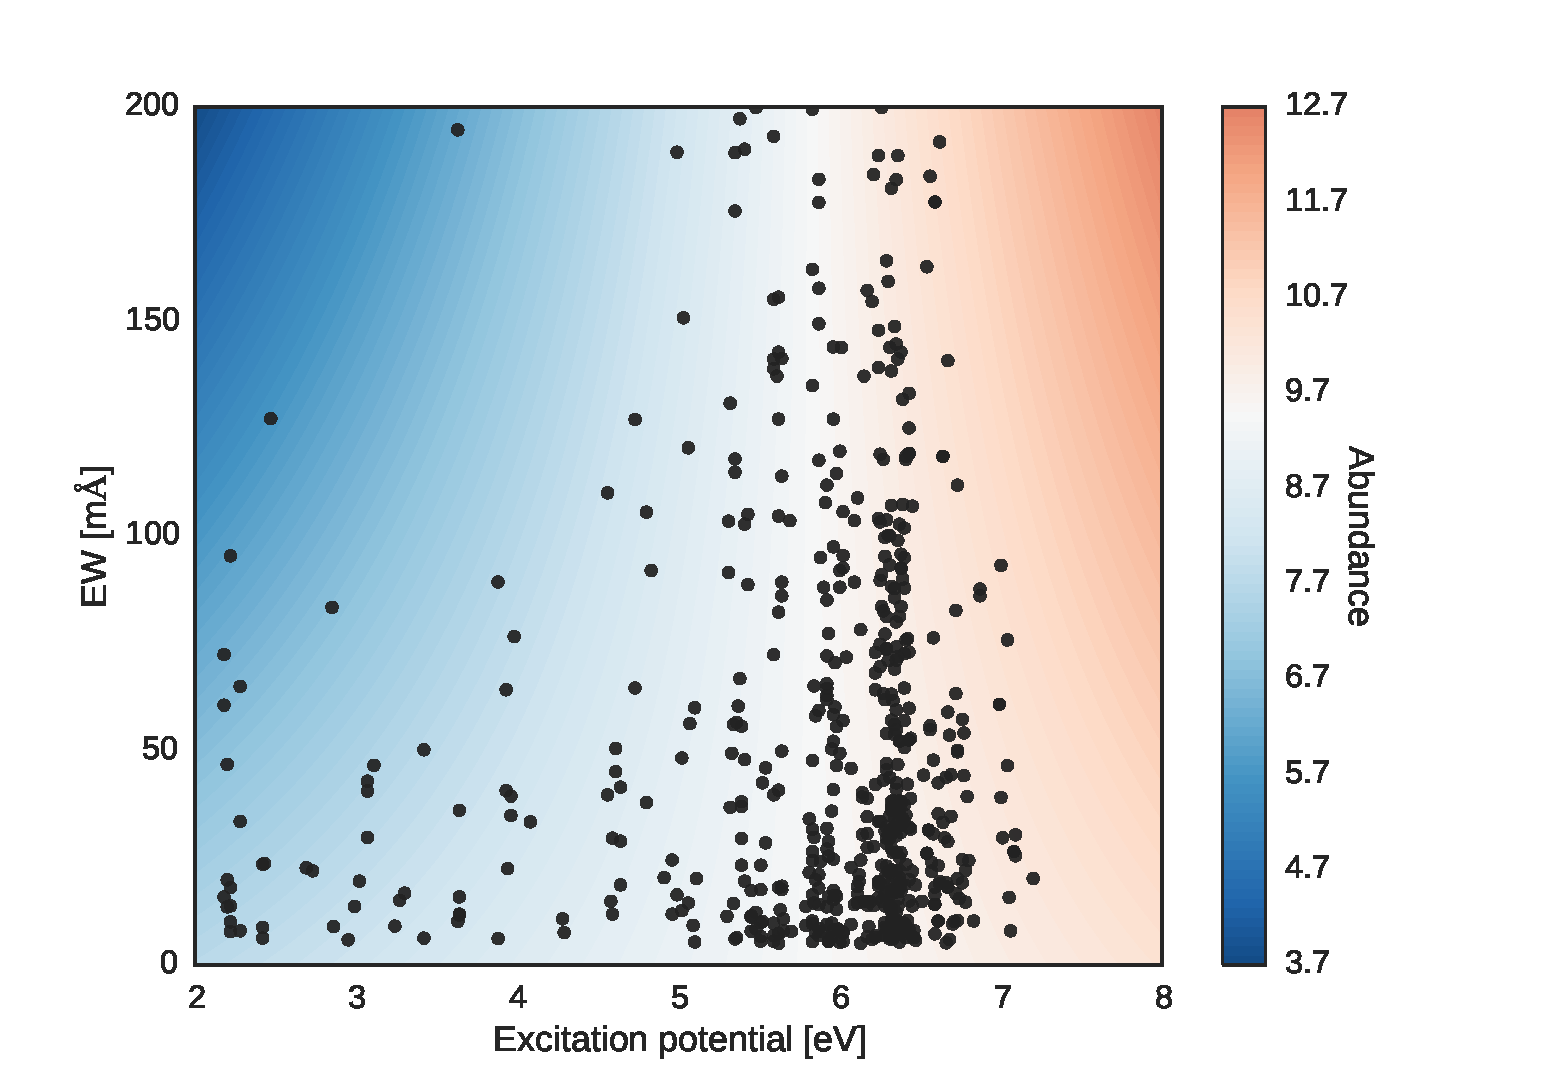
\includegraphics[width=1.0\linewidth]{figures/EWvsEP.pdf}
    \caption{The distribution of Fe I lines with. At the x axis is the
    excitation potential, while the measured EWs for the Sun is shown at the y axis. The
    color scale indicates the abundance before recalibration.}
    \label{fig:Fe1_before_recal}
\end{figure}


\begin{figure}[tpb]
    \centering
    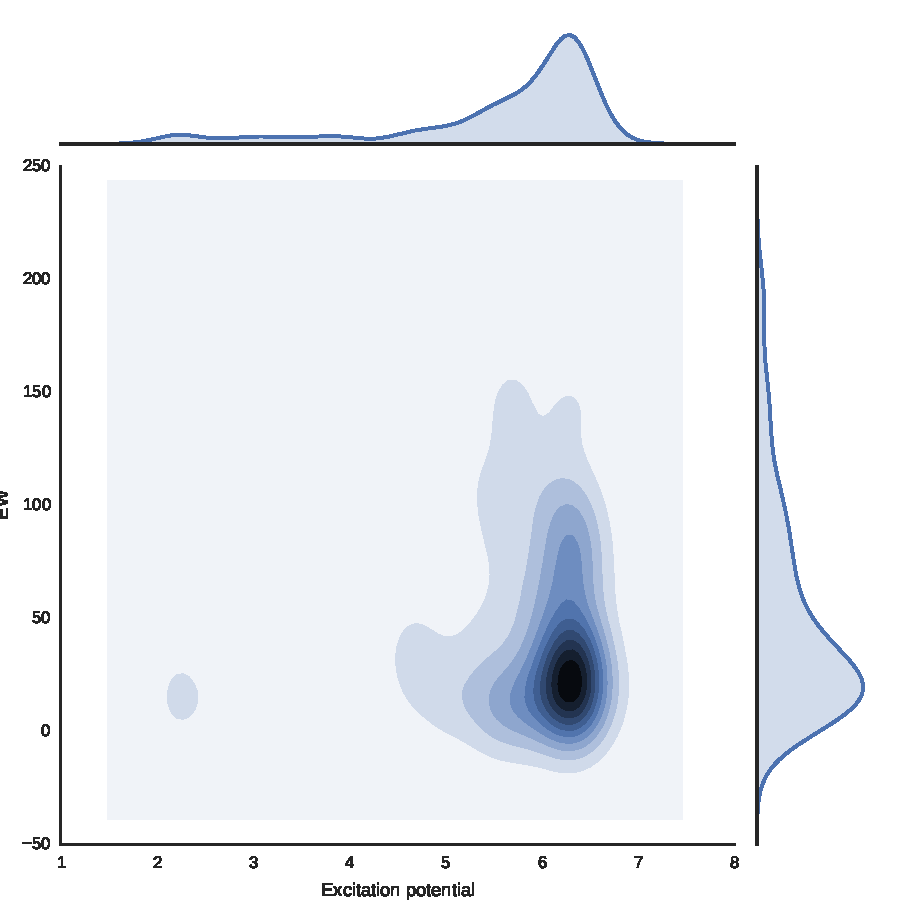
\includegraphics[width=1.0\linewidth]{figures/EWvsEP_cut.pdf}
    \caption{Similar plot as seen in Figure~\ref{fig:Fe1_before_recal}
    but after the recalibration of $\log \mathrm{gf}$. Lines which
    deviates more than 1 dex from the Solar values before recalibration
    are also removed in this plot. The distribution of Fe I lines. At
    the x axis is the excitation potential, while the measured EWs is
    shown at the y axis. The histograms at the top and to the right of
    the plot, show the distribution of the respective axis.}
    \label{fig:Fe1_after_recal}
\end{figure}



\subsection{Deriving parameters with the EW method}
\label{sec:deriving_parameters_with_the_ew_method}

Once the EWs have been measured for all lines in the line list (or as
many as possible), the next step is to derive atmospheric parameters.
Atmosphere models are necessary for computing abundances of the lines.
The literature offers the possibility to choose from a wide variety
of model atmospheres. Models like ATLAS9 \citep{Kurucz1993} and
MARCS \citep{Gustafson2008} are the most used atmospheric models for
derivation of spectroscopic parameters for FGK stars.

Here we use the ATLAS9 models which, for efficiency, are created
in a grid according to effective temperature, surface gravity, and
metallicity. In order to search for final parameters it is necessary to
interpolate models from the grid, thus allowing to look into a finer
grid space \citep[see e.g.][]{Sousa2014}.

For a given atmosphere model, abundances of all the lines in the line
list are calculated. By removing any correlation between the excitation
potential and abundance of all lines (from same element) the effective
temperature is constrained. In a similar way, the micro turbulence can
be constrained be removing any correlation between the reduced EW ($\log
EW$) and abundances, and the surface gravity is found when there is
ionization balance, i.e. the mean abundance of FeI and FeII are equal.
Lastly, the iron abundance comes from calculating the mean of
all the iron abundances.

When there are no longer any correlation, the final atmospheric
parameters are obtained from the atmospheric model to calculate the
given abundances.

In order to find the best atmosphere model, a minimization algorithm
is used based on the downhill simplex method \citep{Press1992} that
searches in the parameter space for the best fitting model. The
convergence criteria for the correlation between excitation potential
and abundances gives a slope less than 0.001, a slope less than 0.002
for the correlation between the reduced EW and the abundances, and a
difference of less than 0.005 between the mean abundances for FeI and
FeII.







\section{Results}
\label{sec:results}


\subsection{Derived parameters for the Sun}
\label{sec:derived_parameters_of_the_sun}

We derive atmospheric parameters for the Sun with the recalibrated line
list. This is a trivial case since the line list is calibrated for the
Sun, but it serves as a consistency test. Additionally, we added noise
to the EW measurements and derived parameters with different cuts in
excitation potential (EP). The noisy EWs follow the procedure from
\cite{Caryel1988}:

\begin{align}
    \sigma \simeq 1.6 \frac{\sqrt{\Delta\lambda\; \mathrm{EW}}}{\mathrm{SNR}},
\end{align}
where $\Delta\lambda=0.1$ and we consider two different signal-to-noise
ratios, 100 and 300. This sigma is used to create a normal distribution
with a mean around the original EW.

\begin{align}
    f(x, EW, \sigma) = \frac{1}{\sqrt{2\pi\sigma^2}} e^{-\frac{(x-EW)^2}{2\sigma^2}}
\end{align}
A new EW is drawn from this distribution and the atmospheric parameters
are derived again. For all EWs we make 10 draws which corresponds to
20 different line lists (2 for each SNR we consider with 10 draws
each). For this 20 line lists we cut in the EP. The cuts are located
at $\SI{5.5}{eV}$ and $\SI{5.0}{eV}$. This gives additionally 40 line
lists, which is a total of 61 including the original line list which at
this point is used as a standard. We derive parameters for all 61 line
lists.


In Figure~\ref{fig:solar_parameters} the parameters are plotted with
different EP cuts in the line list. The horizontal black lines are
the derived atmospheric parameters without noise added to the EWs as
expected. The color shows the two different SNR considered (blue is
SNR at 100, and green is SNR at 300). For a given SNR and EP cut,
the 10 runs were combined to a single value by calculating the mean.
Additionally, we show the 1$\sigma$ standard deviation. A few of the
runs did not converge with our minimization routine. These runs are not
considered in the plot. The derived atmospheric parameters are presented
in Table~\ref{tab:sun}.

\begin{figure}[t!]
    \centering
    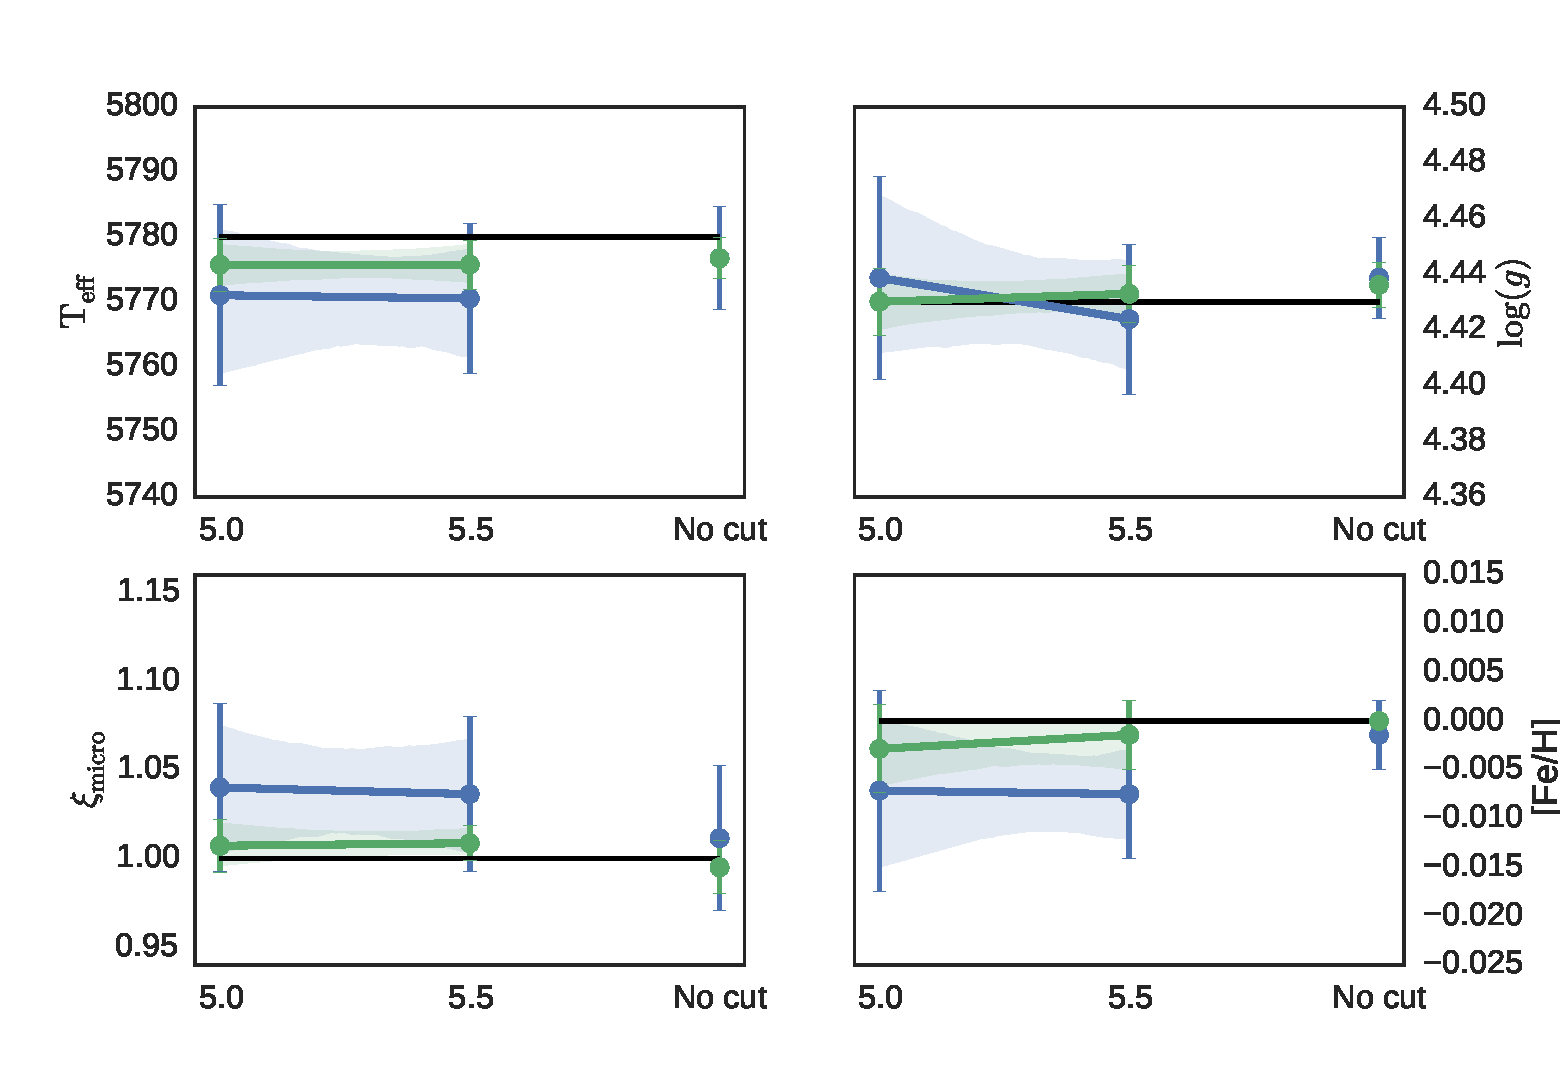
\includegraphics[width=1.0\linewidth]{figures/solar_parameters_10runs.pdf}
    \caption{Derived atmospheric parameters for the Sun. The horizontal
    black lines are the parameters for the calibrated line list, the
    three points shows the mean value of 10 runs with random noise
    added, the blue points is the results for SNR=100, while the
    green points is for SNR=300.}
    \label{fig:solar_parameters}
\end{figure}

By adding noise to the EW measurements and calculate the atmospheric
parameters with different cuts in EP, we see that the final derived parameters
are perfectly compatible with expected values.





\begin{table*}[tb!]
    \caption{The derived parameters for the Sun with two different cuts
    in EP, and with no cut. For all the line lists here, there is noise
    added to the EW measurements.}
    \label{tab:sun}
    \centering
    \begin{tabular}{llllll}
      \hline\hline
        EP cut (eV) &  SNR &  $T_\mathrm{eff}$ (K) &  $\log g$ (cgs)     &  $\xi_\mathrm{micro}$ (km/s) &  [Fe/H]           \\
        \hline
        5.0         &  100 &  $5771 \pm  41$       & $4.44   \pm  0.11$  & $1.04  \pm  0.14$            & $-0.01    \pm 0.03$\\
        5.5         &  100 &  $5770 \pm  34$       & $4.42   \pm  0.08$  & $1.04  \pm  0.13$            & $-0.01    \pm 0.02$\\
        No cut      &  100 &  $5776 \pm  23$       & $4.44   \pm  0.04$  & $1.01  \pm  0.12$            & $-0.00    \pm 0.01$\\
        \hline
        5.0         &  300 &  $5776 \pm  9 $       & $4.43   \pm  0.02$  & $1.00  \pm  0.05$            &  $0.00    \pm 0.00$\\
        5.5         &  300 &  $5774 \pm  11$       & $4.43   \pm  0.04$  & $1.01  \pm  0.04$            & $-0.00    \pm 0.01$\\
        No cut      &  300 &  $5778 \pm  9 $       & $4.44   \pm  0.01$  & $1.00  \pm  0.03$            &  $0.00    \pm 0.00$\\
      \hline
    \end{tabular}
\end{table*}




\subsection{Derived parameters for HD20010}
\label{sec:derived_parameters_of_hd20010}

HD20010 is a well studied F8 subgiant, see e.g.
\cite{Mortier2013,Lebzelter2012}. Therefore, it is a prime object for
our studies, since we want to benchmark results from our new line list
with literature values. To analyse this star we used spectra from
the CRIRES-POP \citep{Lebzelter2012}. The data comes in pieces of
$\SI{50}{\angstrom}$ to $\SI{120}{\angstrom}$. At the time of writing
this paper the data is not yet fully reduced. This is a task the
CRIRES-POP team is working on. However, the data can still be used as it
is after the pipeline reduction. It is already known by the CRIRES-POP
team that the pipeline reduced form of the wavelength calibration is of
poor quality. Most of the spectra are stretched compared to e.g. a model
or a solar spectrum in the same region.

In order to measure the EWs of the lines in our line list, the correct
absorption lines need to be identified. This was done by plotting the
spectra for HD20010, a solar spectrum (the parameters are close enough
so we can use the Sun as a reference), an observed telluric spectrum
from the TAPAS web page \citep{Bertaux2014}, and the lines from our
line list in the region we are looking at. The pieces of spectra are
shifted in radial velocity as well. A software was developed that
plots everything and calculate the cross correlation function of the
model (in this case the Sun), and the telluric spectra\footnote{The
software (plot\textunderscore{}fits) is open source and can be found
here: \url{https://github.com/DanielAndreasen/astro_scripts}}. The two
CCFs are fitted with a Gaussian, and the mid point is the RV. These two
RVs are used to shift the model and telluric respectively. The lines
from our line list are shifted with the same RV as for the model.
Figure~\ref{fig:plot_fits} shows an example of this.

\begin{figure*}[tbp!]
    \centering
    \includegraphics[width=1.0\linewidth]{figures/plot_fits.pdf}
    \caption{The middle plot shows a piece of HD20010 (black), the model
    spectrum, in this case the Sun (green), a telluric spectrum (red), and two
    lines from our line list (magenta vertical lines). The plot to the left
    shows the CCF of the Sun with a fitted Gaussian. The right plot shows the
    same as the one to the left, but for the telluric spectrum.}
    \label{fig:plot_fits}
\end{figure*}

Once the lines are identified the EWs were measured with the splot
routine in IRAF. The reason not to choose ARES for this task was because
of the relative poor wavelength calibration at the moment.

The derived parameters for HD20010 for the full line list
are overestimated compared to literature values, see e.g.
\citet{Mortier2013,Gonzalez2010}. \cite{Gonzalez2010} use the same
method as us, but for an optical spectra, and derive the following
atmospheric parameters: $T_\mathrm{eff}=6170\pm33\,\si{\kelvin}$,
$\log g=3.93\pm0.02$, $\xi_\mathrm{micro}=1.70\pm0.09\,\si{km/s}$,
and [Fe/H]=$-0.206\pm0.025$. To overcome this problem we tried
to remove lines above different EPs and re-determine the stellar
atmospheric parameters. In this process we did not remove any of the
FeII lines (we were only able to measure the EWs of 5 lines out of
the 13 from the solar case). The reason not to remove the FeII lines
is, that they are essential to determine the surface gravity from the
ionization balance. As it turned out, 5 lines were too few, and we
fixed the surface gravity to the value found in \cite{Gonzalez2010}.
Figure~\ref{fig:HD20010_parameters_cuts} shows the results from this
exercise. A second degree polynomial is fitted for the effective
temperature, iron abundance, and the micro turbulence with the
95\% confidence interval. At a cut at $\SI{5.5}{eV}$ and below
the atmospheric parameters gets close to the values derived from
\cite{Gonzalez2010} which is plotted as a horizontal black line. The
exact values can be seen in Table~\ref{tab:hd20010}.


\begin{table*}[htb!]
    \caption{The derived parameters for HD20010 at different EP cut. $\log g$
        were fixed at 3.93 for all calculations. The literature value are from \cite{Santos2004}.}
    \label{tab:hd20010}
    \centering
    \begin{tabular}{lllll}
      \hline\hline
        EP cut (eV) & $T_\mathrm{eff}$ (K) & $\xi_\mathrm{micro}$ (km/s) & [Fe/H]               \\
      \hline
        Literature  & $6170 \pm  33$       & $1.70 \pm 0.09$             & $-0.21 \pm 0.03$      \\
      \hline
        5.0         & $6112 \pm 121$       & $0.78 \pm 0.08$             & $-0.25 \pm 0.44$      \\
        5.1         & $6067 \pm 209$       & $1.39 \pm 0.17$             & $-0.29 \pm 0.74$      \\
        5.2         & $6093 \pm 196$       & $1.37 \pm 0.16$             & $-0.29 \pm 0.71$      \\
        5.3         & $6096 \pm 196$       & $1.37 \pm 0.16$             & $-0.29 \pm 0.73$      \\
        5.4         & $6294 \pm 353$       & $2.00 \pm 0.30$             & $-0.27 \pm 1.52$      \\
        5.5         & $6337 \pm 558$       & $2.14 \pm 0.49$             & $-0.26 \pm 2.48$      \\
        5.6         & $6367 \pm 714$       & $2.21 \pm 0.63$             & $-0.26 \pm 3.33$      \\
        5.7         & $6621 \pm 248$       & $2.18 \pm 0.20$             & $-0.20 \pm 1.35$      \\
        5.8         & $6624 \pm 241$       & $2.17 \pm 0.19$             & $-0.20 \pm 1.31$      \\
        5.9         & $7000 \pm 218$       & $2.09 \pm 0.09$             & $-0.11 \pm 1.29$      \\
        6.0         & $6999 \pm 181$       & $2.08 \pm 0.08$             & $-0.10 \pm 1.06$      \\
        No cut      & $7150 \pm 467$       & $2.99 \pm 0.30$             & $-0.09 \pm 3.04$      \\
      \hline
    \end{tabular}
\end{table*}



\begin{figure}[tpb!]
    \centering
    \includegraphics[width=1.0\linewidth]{figures/HD20010_parameters_cuts.pdf}
    \caption{Atmospheric parameters for HD20010. In the top panel is
    the effective temperature. The middle panel is the iron abundance,
    and the bottom panel is the micro turbulence. The parameters are
    derived with different cuts in EP. Here the horizontal black lines
    are literature values. The parameters for the full line list are
    plotted to the right for all three plots. The shaded areas are the
    95\% confidence interval for the fit.}
    \label{fig:HD20010_parameters_cuts}
\end{figure}






\begin{acknowledgements}
D.T.A, S.G.S, E.D.M and N.C.S  acknowledge support from the Funda\c{c}\~ao
para a Ci\^encia e Tecnologia, FCT (Portugal) in the form of grants
SFRH/BPD/76606/2011, SFRH/BPD/47611/2008, and SFRH/BPD/70574/2010,
respectively. PF acknowledges support by Funda\c{c}\~ao para a Ci\^encia
e a Tecnologia (Portugal) through Investigador FCT contracts of
reference IF/01037/2013 and POPH/FSE (EC) by FEDER funding through
the program ``Programa Operacional de Factores de Competitividade -
COMPETE''.

This research made use of the SIMBAD database operated at CDS,
This Strasbourg (France) and the Encyclopaedia of Extrasolar Planets.\\
This work also made use of the IRAF facility.


\end{acknowledgements}






\newpage
\bibliography{thesis}
\bibliographystyle{astron}
\nocite*{}

\end{document}
